\documentclass{article}

\usepackage{graphicx}
\graphicspath{ {./images} }

\title{Ch. 15 CW \#2 Solutions}
\author{Principles of Microeconomics}
\date{\today}

\begin{document}

\maketitle

\section*{15.2. The Competitive Firm's Supply Curve}

\begin{enumerate}

\item A firm will shut down temporarily if $P < AVC$. If $P < AVC$, then the revenue from producing the typical unit is less than the  variable cost of producing the typical unit. That means the firm is losing more money producing than it would by shutting down. In the short run, fixed costs are unrecoverable whether or not the firm shuts down, so they don't factor into the firm's shut down decision.

\item A firm will exit a market if $P < ATC$. If $P < ATC$, then the firm's profits are negative. If profits are negative, then the firm will exit the market in the long run.

\end{enumerate}

\section*{15.3. The Competitive Market's Supply Curve}

\begin{enumerate}

\setcounter{enumi}{2}
\item 

	\begin{enumerate}
	
	\item The technological advance lowers fixed costs, so it lowers every firm's ATC curve. If ATC decreases, then profits increase. When profits become positive, firms will enter the market. That shifts supply right which in turn drives price and profits back down. Firms will enter until profits are back to zero.
	
	\item The increase in wages increases variable costs, so it raises every firm's ATC curve. If ATC increases, then profits decrease. When profits become negative, firms will exit the market. That shifts supply left which in turn drives price and profits back up. Firms will exit until profits are back to zero.
	
	\item For the same reasons as in (b), firms will exit the industry until profit returns to zero.
	
	\end{enumerate}
	
\newpage
	
\item \phantom{x}

	\begin{center}
	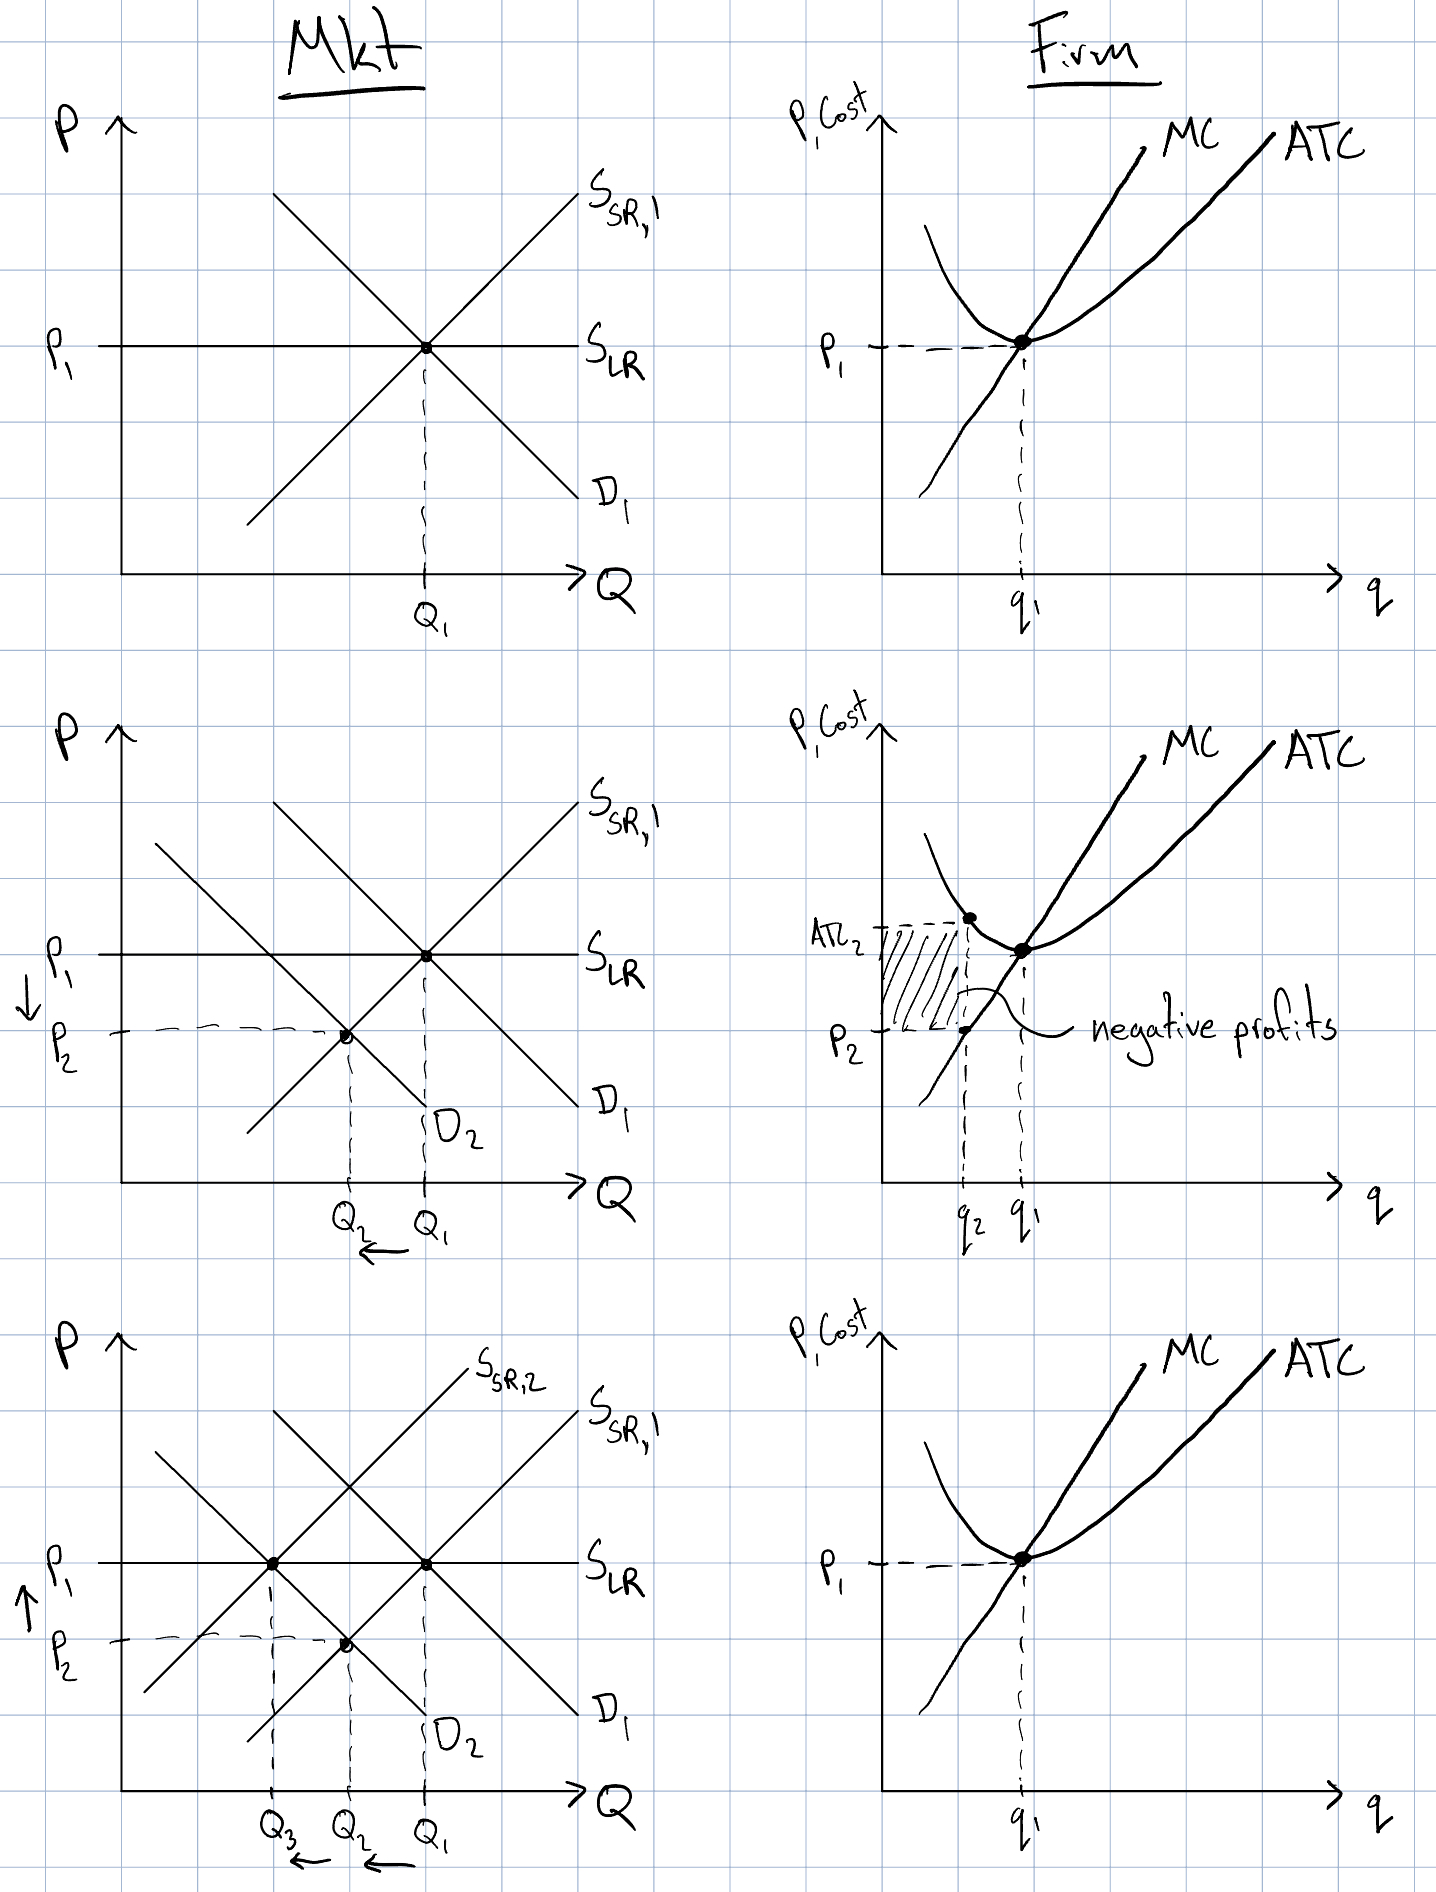
\includegraphics[width = \textwidth]{q4}
	\end{center}

\end{enumerate}

\end{document}